\begin{figure}[H]
    \centering
    \begin{tikzpicture}
        \pgfplotsset{
            width=0.4\textwidth,
            height=0.4\textheight
        }
        \begin{axis}
            [
                xbar=2pt,
                legend style={at={(0.5,-0.15)}, anchor=north,legend columns=-1},
                bar width = 5pt,
                xlabel= DEC (Joules),
                xmin=0,xmax=1100,
                symbolic y coords = {
                    IPG, 
                    LHM, 
                    SCAP, 
                    SCAPI, 
                    {Clamp (W)}, 
                    {Plug (W)},
                    RAPL,
                    {Clamp (L)},
                    {Plug (L)}},
                    ytick={IPG,LHM,SCAP,SCAPI,{Clamp (W)},{Plug (W)},RAPL,{Clamp (L)},{Plug (L)}},
                    % xbar=1pt
            ]
            \addplot coordinates { 
                (484,IPG)
                (479,LHM)
                (482,SCAP)
                (659,SCAPI)
                (377,{Clamp (W)})
                (549,{Plug (W)})
                (253,RAPL)
                (166,{Clamp (L)})
                (289,{Plug (L)})
                };
            \addplot coordinates { 
                (420,IPG)
                (431,LHM)
                (455,SCAP)
                (565,SCAPI)
                (345,{Clamp (W)})
                (482,{Plug (W)})
                (536,RAPL)
                (457,{Clamp (L)})
                (635,{Plug (L)})
                };
            \legend{FR, MB}
            \end{axis}
        \end{tikzpicture}
    \caption{The DEC for DUT 1, where both benchmarks were compiled on oneAPI} \label{fig:dut-1-compare-mi}
\end{figure}
